\documentclass{article}
\usepackage{graphicx}
\usepackage{enumitem}
\usepackage{amsfonts}
\usepackage{hyperref}
\usepackage{amsmath}
\usepackage[dvipsnames]{xcolor}
\usepackage{listings}
\usepackage{tcolorbox}
\tcbuselibrary{listings} 
\usepackage{listings}
\usepackage[left=1in, right=1in, top=1in, bottom=1.25in]{geometry}
\usepackage{tikz}
\usepackage[utf8]{inputenc} 
\tcbuselibrary{theorems} 
%%%%%pour les bordure de codes C


\begin{document}

\begin{titlepage}
    \centering
    \Huge\bfseries
    Munificence

    \vspace{3cm}
    
\begin{figure}[ht]
    \centering
    \includegraphics[width=0.70\linewidth]{projMunificence.jpg}
    \caption{\large Pièces du plateau de jeu}
    \label{fig:projMunificence}
\end{figure}
    
    
    \vspace{3cm}
    
    \Large
    Projet réalisé par 
    Oussama LAMRID, Mathis PEREIRA PEDRO 
    
    \vspace{1cm} 
    
    \Large 
    Encadré par Monsieur Vinh-Thong Ta
    
    \vspace{1cm}

    
    \Large
    ENSEIRB-MATMECA 2023-2024
    
    \vspace{0.5cm} 

    
    \vfill % Remplissage de l'espace vertical restant
    
   
\end{titlepage}



\renewcommand{\contentsname}{Sommaire}

\tableofcontents

%Le sommaire est pour l'instant qu'en état de brouillon n'hésite pas à me dire ce que tu veux ajouter/supprimer
%
\newpage
\section{Introduction}
\hspace{1em}Dans le cadre de notre première année de cycle d'ingénieur à l'ENSEIRB MATMECA en filière informatique, nous avons pu découvrir le travail sur la longue durée grâce à ce premier projet en langage C, ainsi que le travail en groupe. Ce projet nous a permis de mettre en œuvre et d'élargir nos compétences en programmation dans ce langage, ainsi que de développer notre utilisation de notre environnement de travail.


\section{Objectifs du Projet}
\subsection{Sujet}
\vspace{1em}Le sujet mis à notre disposition est une version altérée du jeu de plateau Splendor. Le but est de recréer le jeu de telle manière à ce que nous fassions jouer des joueurs programmés par nos soins au jeu que nous avons nous-mêmes créé.

\subsection{Contraintes et Objectifs}

\subsubsection{Contraintes}
\hspace{1em} Les contraintes sur ce projet étaient peu nombreuses, mais celles mises en place nous obligeaient à réfléchir à des définitions qui soient viables dans le temps. Effectivement, ce projet fonctionnait sous forme d'achievements, ce qui signifiait qu'une fois passés les achievements, nous pouvions avancer. Ainsi, il fallait réfléchir à des structures assez souples qui soient prêtes à être changées sans avoir à tout réécrire. De plus, il nous était impossible de modifier les fichiers .h initialement présents. Ces deux obligations sont intéressantes car elles permettent une modélisation du code à laquelle nous serons confrontés plus tard.

\subsubsection{Objectifs}
\hspace{1em} Les objectifs de ce projets étaient nombreux mais malheureusement pas tous atteints. Tout d'abord le travail de groupe, en effet l'apprentissage du travail de groupe est un des objectifs du projet. Il y avait aussi la volonté d'aller le plus loin possible dans les achievements. À cela s'ajoute l'envie de mieux définir son environnement de travail et enfin l'amélioration de nos compétences en C. 

\section{Gestion du Projet}
 
\subsection{Outils}


%pas sur de la pertinence de cette section. 

\subsubsection{Git}

\hspace{1em}Git est un outil permettant de partager nos fichiers de code facilement et rapidement sur un dépôt commun distant. Nous avons pu apprendre à partager un dépôt et à le gérer afin de le maintenir clair pour tous les deux. Il nous a aussi permis d'approfondir le cours d'environnement de travail  en traitant de cette partie en configurant Git sur nos machines respectives, ainsi qu'en abordant les conflits de merging que nous avons rencontré plusieurs fois. 

\subsubsection{La Forge}

\hspace{1em} La Forge était notre dépôt commun distant sur lequel nous envoyions nos fichiers via Git. Elle servait également à tester notre code. Les tests écrits sur cette dernière nous indiquaient si la solution au problème proposée était viable et répondait au cahier des charges, du moins pour les tests qu'elle appliquait à notre code.

\subsection{Répartition des tâches}

\hspace{1em} Pour un tel travail de groupe il était nécessaire de partager le travail afin de ne pas perdre de temps et être le plus efficace possible ainsi qu'éviter tout conflit.  

\subsubsection{La comunication}


\subsubsection{Répartition binaire}

\hspace{1em}La gestion de ce projet se faisait plutôt naturellement car celui-ci était construit de manière binaire. On peut le voir clairement sur le schéma de l'architecture du projet \ref{schema}. L'un pouvait travailler sur les builders et la guilde pendant que l'autre se penchait sur les \emph{tokens} et le \emph{marché}. Ainsi, Mathis s'est occupé de la partie traitant des \emph{builders} dans sa globalité, tandis qu'Oussama s'est occupé des \emph{tokens}.
\subsubsection{Travail commun}

\hspace{1em} Toutefois, nous ne travaillions pas uniquement chacun de notre côté. Il était important d'échanger pour expliquer à l'autre l'idée que nous voulions mettre en place pour que le projet ait un minimum de sens dans sa globalité. De plus, dans certains cas, on se rendait compte en expliquant des potentielles erreurs ; parfois, l'autre soulignait des cas limites non considérés. De plus, nous avons aussi été amenés à travailler sur le même document et sur les mêmes parties du projet \emph{player} et le fichier \emph{project} d'où la nécessité de la communication. 


\subsubsection{Empiètement}

\hspace{1em} Effectivement, dans certaines situations, nous devions travailler sur les mêmes fichiers, comme lors de la boucle de jeu (dans le fichier \emph{project.c}) ou dans la définition du joueur (dans le fichier \emph{player.c}). Dans ces cas-là, nous pouvions être amenés à créer deux fichiers différents pour accomplir des tâches similaires et les fusionner par la suite. Bien que ce ne soit pas la méthode la plus optimale, nous avons pu échanger nos idées et tirer le meilleur des deux côtés. 

\section{Développement du Projet}
\vspace{1em}
\subsection{Compilation séparée}

\hspace{1em}Durant ce travail, pour que cela soit plus pratique et compréhensible, nous avons travaillé sur plusieurs fichiers différents. Cela nous a permis de pratiquer la programmation modulaire et d'éviter également des conflits sur Git. Cependant, travailler sur plusieurs fichiers implique de devoir compiler plusieurs fichiers en même temps en raison de leurs dépendances mutuelles, d'où le recours à la compilation séparée et la nécessité de n'avoir qu'un seul main. 

\subsubsection{L'architecture du projet}
 
%%architecture du projet
\hspace{1em}Comme expliqué précédemment, le projet s'étalait sur plusieurs fichiers. Il était découpé de manière symétrique, ce qui permettait à chacun de travailler sur sa partie.

\hspace{1em}


%%
\begin{minipage}{0.6\textwidth} \label{schema}
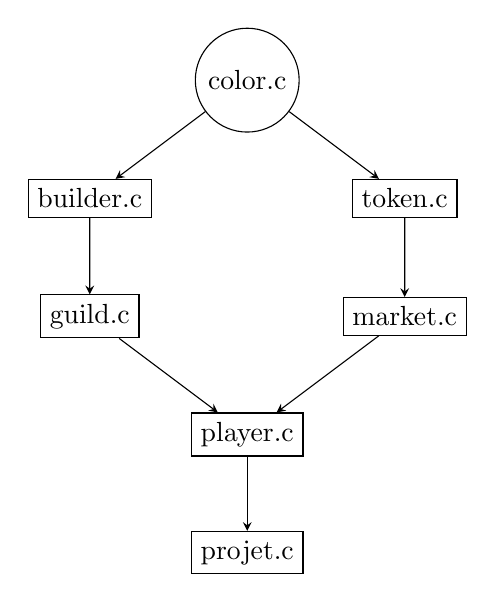
\begin{tikzpicture}[->,>=stealth,level/.style={sibling distance = 4cm/#1,
  level distance = 1.5cm}]
\node [circle,draw] (color) {color.c}
  child {node [rectangle,draw] (builder) {builder.c}
    child {node [rectangle,draw] (guild) {guild.c}
    }
  }
  child {node [rectangle,draw] (token) {token.c}
    child {node [rectangle,draw] (market) {market.c}
    }
  };
% Définir player.c et projet.c une seule fois
\node [rectangle,draw] (player) at (0,-4.5) {player.c}
  child {node [rectangle,draw] (projet) {projet.c}};

% Dessiner les chemins
\draw[->] (guild) -- (player);
\draw[->] (market) -- (player);
\end{tikzpicture}
\end{minipage}
%%%
\begin{minipage}{0.4\textwidth}

Notre projet implique la création d'un fichier project.c, dans lequel nous établissons la boucle de jeu permettant à un joueur de jouer. Ce fichier dépend du fichier player.c. Lorsque le joueur prend des jetons (tokens) du marché et embauche des architectes (builders) depuis la guilde, player.c fait appel aux fichiers market.c et guild.c qui eux mêmes font appel à respectivement builder.c et respectivement token.c. Le fichier market.c gère les jetons, nécessitant ainsi le fichier token.c, tandis que guild.c gère les architectes, faisant appel au fichier builder.c. Ces deux derniers fichiers dépendent, pour leur fonctionnement, du fichier color.c qui détermine les couleurs des \emph{tokens} et \emph{builers}.




\end{minipage}

\subsubsection{La compréhension des différents fichiers}

\hspace{1em} Avant de commencer le codage, il était essentiel de comprendre la différence entre un fichier .c et un fichier .h pour ne pas écrire de code dans un fichier .h notamment, un concept nouveau pour nous . Nous avons appris que le fichier .h doit contenir uniquement les prototypes de fonctions et les informations nécessaires à la compilation des fichiers .c. Il est crucial de gérer correctement les dépendances entre les fichiers, en veillant à inclure uniquement les fichiers .h nécessaires et à éviter les inclusions multiples du même fichier. De plus, il faut s'assurer que les dépendances ne créent pas de conflits ou de références croisées.


\subsubsection{Gestion des définitions inter fichiers}

\vspace{1em}
\hspace{1em} Comme nous utilisons des structures dans des fichiers distincts il est nécessaire de pouvoir y accéder facilement. Deux options existaient, les variables externes telle que le \emph{market} et le choix de travailler avec des pointeurs comme pour la \emph{guilde}.\\ 

Maintenant que nous avons plusieurs fichiers, il est nécessaire de les compiler pour voir leur état. Cette étape peut se révéler fastidieuse si on doit écrire la compilation de chaque fichier à chaque fois. On introduit donc le Makefile.

\subsubsection{Makefile}

\hspace{1em} Le Makefile permet directement à l'aide d'une commande préalablement écrite de compiler tous les fichiers demandés et donc gagner du temps et de l'énergie. Comme nous pouvons l'observer sur la figure \ref{fig:project}.
%%%%
\begin{figure}[ht]
    \centering
    \includegraphics[width=0.40\linewidth]{Make Project.png}
    \caption{Compilation Makefile (make project)}
    \label{fig:project}
\end{figure}
%%%%

\vspace{1em} Lors de l'écriture du Makefile, il est nécessaire de faire attention aux dépendances entre les fichiers. Vérifier que chaque fichier.o nécessaire est présent. Par exemple pour la compilation de  project.c, nous avons besoin de tous les fichiers d'où la présence de tous les fichiers .o 

\newpage


\vspace{1em} Cependant avec cette commande nous n'avons pas encore compiler. Les trois premières lignes servent à générer les fichiers .o de chaque répertoire. Le -I lui permet de faire le lien entre les dépendances. En effet les fichiers dans \emph{tst} dépendent de fichiers de src. C'est  pourquoi il faut indiquer à la machine qu'elle doit aller chercher ces fichiers ailleurs avec -I \textdollar(SRC). Dans le cas du make project le \textdollar(PROJ) vérifier l'éxistence des fichiers .o dans \textdollar(PROJ) et il va les générer s'ils ne sont pas présents. Enfin le \textdollar(CC) et \textdollar(CFLAGS) sont les options de compilations précédemment définies dans le Makefile, c'est d'ailleurs dans ce dernier qu'est placer le -I \textdollar(SRC).
%%%

\begin{tcolorbox}[colback=gray!10,colframe=white!75!black]
\begin{lstlisting}[language=C, caption={Commande de compilation}, label={lst:exemple1-c}]
%.o: $(SRC)/%.c
	$(CC) -c $(CFLAGS) $<

%.o: $(TST)/%.c
	$(CC) -c -I$(TST) $(CFLAGS) $<

%.o: %.c
	$(CC) -c $(CFLAGS) $<

test: $(OBJ)
	$(CC) $(CFLAGS) $(OBJ) -o test

project: $(PROJ)
	$(CC) $(CFLAGS) $(PROJ) -o project

\end{lstlisting}
\end{tcolorbox}
\vspace{1em} En conclusion, le Makefile s'est révélé être un outil précieux, nous permettant de gagner un temps considérable lors de la compilation des fichiers. Son utilité réside dans sa praticité et sa facilité d'exécution, même si sa compréhension initiale peut s'avéra un peu complexe.

\subsection{Gestion de la mémoire}

\hspace{1em} Comme le projet s'étalait sur plusieurs fichiers, nous ne pouvions pas uniquement travailler avec des variables statiques. Nous avons donc dû trouver des alternatives permettant d'y accéder même dans les autres fichiers. 

\

\subsubsection{Les pointeurs}
\vspace{1em}
\hspace{1em}L'utilisation de pointeurs était particulièrement adaptée à ce projet, car ils offrent un accès direct à l'adresse mémoire des variables, indépendamment du fichier dans lequel on se trouve. La seule contrainte était d'inclure le pointeur de la variable concernée en tant que paramètre de la fonction. Ainsi, dans la boucle de jeu et dans le fichier dédié à la définition des joueurs, il suffisait de manipuler uniquement les pointeurs de la guilde et des joueurs.

Prenons l'exemple de la structure \emph{builder\_t}, un type abstrait qui ne peut être défini que dans le fichier builder.c. Cela signifie que dans les autres fichiers, les builders ne peuvent être manipulés qu'à travers des pointeurs, à l'exception de builder.c. En conséquence, la fonction \emph{make\_builder}, qui est utilisée pour créer des builders, renvoie des pointeurs sur la structure \emph{builder\_t}.

%%%
\begin{tcolorbox}[colback=gray!10,colframe=white!75!black]
\begin{lstlisting}[language=C, caption={La fonction \text{make\_builder}},label={lst:exemple0-c}]
struct builder_t *make_builder(unsigned int index)
{ 
  return &builders[index];    
}
\end{lstlisting}
\end{tcolorbox}

%%%

\subsubsection{Les erreurs de segmentations}

\hspace{1em} L'erreur de segmentation a lieu quand on cherche à atteindre un espace mémoire qui n'est pas accessible par la mémoire. Nous y avons eu plusieurs fois affaire notamment lors de l'utilisation des \emph{builders} et dans le parcours de la \emph{guild}. Cela pouvait arriver quand les \emph{builders} n'étaient pas initialisés ou un parcours de tableau qui dépassait ce son dernier indice. La situation délicate au premier abord c'est qu'il n'empêche pas la compilation du fichier. Ils n'apparaissent que lors de l'exécution et on ne sait pas à quel endroit dans cette dernière. 

\subsubsection{Le debbugage}

\vspace{1em}

 

\hspace{1em} Pour identifier les problèmes de segmentations, nous avons dû procéder à du debuggage. Dans un premier temps avons d'abord utilisé la fonction \emph{printf}  pour examiner les variables et localiser l'erreur dans le code. Cependant, cette méthode a montré ses limites, en particulier lors de la mise au point de la boucle de jeu. Nous avons donc dû recourir à des outils de débogage. L'outil principal que nous avons utilisé était LLDB, un débogueur initialement développé pour les systèmes Apple. Comme illustré dans la figure \ref{fig:lieux erreur}, cet outil indique l'emplacement précis de l'erreur et le fichier concerné.



\begin{figure}[ht]
    \centering
    \includegraphics[width=0.45\linewidth]{Lieux erreur.png}
    \caption{Lieux de l'erreur}
    \label{fig:lieux erreur}
\end{figure}
\newpage
Toutefois on ne peut pas se contenter de cette unique information. Avec ce debuggeur, nous pouvons observer l'état des variables à l'instant de l'erreur via la commande \emph{p}. Ainsi on peut voir sur l'exemple d'un \emph{buider} mal configuré sur la figure \ref{fig:print lldb}. On peut donc en déduire que même si l'erreur de segmentation provient de la fonction \emph{possible} le souci vient plutôt de l'initialisation des builders. Cependant pour le dernier bug résolu ces outils ne suffisaient pas. Nous avons utilisé la fonction \emph{rbreak} qui permet de s'arrêter à la valuation d'une fonction ou encore la compilation ligne par ligne avec la commande \emph{n}. 


\begin{figure}[ht]
    \centering
    \includegraphics[width = 0.5 \linewidth]{printlldb.png}
    \caption{État des variables lors de l'erreur}
    \label{fig:print lldb}
\end{figure}


%le choix des définitions

\subsection{Le choix des définitions}

\vspace{1em}


\hspace{1em}Pour caractériser les élements essentiels dans notre jeu tels que les \emph{tokens} et les \emph{builders}, il est essentiel de disposer d'informations telles que la couleur et les ressources sur un token ou bien les points de victoires  sur un builder,. Afin de simplifier les fonctions utilisées en minimisant le nombre de paramètres, nous faisons usage de structures.
%%%%%%les tokens

\subsubsection{Les tokens}

\begin{figure}[ht]
    \centering
    \includegraphics[width=0.5\linewidth]{tokens.png}
    \caption{La forme des jetons colorés dans le jeu.}
    \label{fig: LA FORME DES TOKENS  }
\end{figure}


\hspace{1em} Un token représente un ensemble de ressources, or on utilise dans notre jeu deux types  de tokens: les tokens simples avec un nombre de ressources vaut 1 et d'autres complexes avec un nombre de ressources vaut 2, afin de caracteriser les tokens nous définissons une première structure nommée \text{token\_t}.


%%%%
\begin{tcolorbox}[colback=gray!10,colframe=white!75!black]

\begin{lstlisting}[language=C, caption={La structure caracterisant un  Token}, 
label={lst:exemple19-c}]
struct token_t {
  unsigned int c[NUM_COLORS];
};
\end{lstlisting}
\end{tcolorbox}
%%%

La structure est sous forme d'un tableau d'entiers avec chaque indice qui represente une couleur(avec l'ordre suivant: BLACK BLUE GREEN RED WHITE) et la case correspondante represente les ressources de ce couleur sur ce token.\\ 

\vspace{1em}exemple1: un token simple de couleur noir(BLACK) représenté comme suivant \text{token\{1,0,0,0,0\}}.\\
 
\vspace{1em}
exemple2: un token complexe de couleur vert(GREEN) représenté comme suivant \text{token\{0,0,2,0,0\}}

\subsubsection{Le Market}
%%%%
 Le marché représente l'endroit où les jetons sont rendus disponibles aux joueurs pour l'achat durant la partie. Il prend la forme d'un plateau. Cf le vrai plateau de jeu sur la figure \ref{fig:PLATEAU}
\begin{figure}[ht]
    \centering
    \includegraphics[width=0.4\linewidth]{plateau.png}
    \caption{Le market}
    \label{fig:PLATEAU}
\end{figure}
%%%

Notre market est donc  représenté par une matrice de 5x5, qui est remplie de jetons.
\begin{tcolorbox}[colback=white!5,colframe=white!75!black]

\begin{lstlisting}[language=C, caption={le plateau}, label={lst:exemple6-c}]

struct token_in_market notre_market[5][5];
\end{lstlisting}
\end{tcolorbox}
%%%
or le token dans le market a plusieurs caracteristiques telles que son état et sa position (i,j) dans le plateau d'où l'implémentation suivante pour la structure du market.

\begin{tcolorbox}[colback=gray!10,colframe=white!75!black]

\begin{lstlisting}[language=C, caption={la structure token\_in\_market}, label={lst:exemple7-c}]
struct point
{
    int i;
    int j;
};

struct token_in_market{
    struct token_t token;
    struct point pos ;
    int etat;                            
    int a;                        
    unsigned int n;             
};
\end{lstlisting}
\end{tcolorbox}
\vspace{2em}
\hspace{1.5em}La collecte des jetons par un joueur est soumise à une contrainte imposée par l'achievement1. Selon cette contrainte, les jetons choisis doivent se trouver dans un état connexe sur le plateau. Pour respecter cette exigence, nous avons mis en place la fonction \texttt{pick\_tokens}. Cette fonction a été conçue spécifiquement pour garantir que les jetons sélectionnés sont dans un état connecté sur le plateau de jeu.



%%%%%
%%%%
%%%%%les builders
\subsubsection{Les builders}



    Un \emph{builder}, dans le contexte du jeu, représente un élément que les joueurs peuvent recruter en échange d'un certain coût en ressources. Une fois recruté, cet architecte est capable de générer un certain nombre de ressources. Les \emph{builders} se distinguent les uns des autres par leur \emph{index}, ils possède un niveau défini sur une plage allant de 0 à NUM\_LEVELS , ils octroient un certain nombre de points de victoire au joueur qui les possède. En général, un \emph{builder} de niveau plus élevé a tendance à rapporter davantage de points de victoire.

    
   
\begin{tcolorbox}[colback=gray!10,colframe=white!75!black]

\begin{lstlisting}[language=C, caption={La structure caracterisant un Builder}, 
label={lst:exemple2-c}]
struct builder_t
{
  unsigned int level;
  unsigned int index;
  unsigned int points;
  struct buildcost_t requires;
  struct buildcost_t provides;
};
\end{lstlisting}
\end{tcolorbox}
%%%%%
\vspace{10pt}
Le  coût d'embauche (requires) et la  capacité de production (provides) sont mises sous forme d'une structure à deux composantes,
par exemple le composant provides d'un builder qui a une capacité de production de 3 ressources noires (3B) est sous la forme \(\{0,3\}\)
    
    
%%
\begin{tcolorbox}[colback=gray!10,colframe=white!75!black]

\begin{lstlisting}[language=C, caption={la structure buildcost\_t} , label={lst:exemple3-c}]
struct buildcost_t {
  enum color_t c;       
  unsigned int n;       
};
\end{lstlisting}
\end{tcolorbox}

\hspace{1em} Tout comme les \emph{tokens}, les \emph{builders} sont rangés mais dans une \emph{guilde}. Elle doit permettre de savoir si un builder est disponible à l'achat. 

\subsubsection{La Guilde}
\vspace{1em}
\hspace{1em}
La guilde représente l'endroit où les architectes (builders) sont rendus disponibles aux joueurs pour l'embauche au cours du jeu. Elle dispose d'un tableau de \emph{MAX\_BUILDERS} éléments de la structure \emph{guild\_one\_t} qui permet de caractériser un builder dans la guilde. Nous avons décidé de prendre la structure \emph{guild\_one\_t} car elle permet de déterminer imédiatement si un builder est disponible à l'achat avec le champ \emph{struct guild\_one\_t.state}. Effectivement nous l'initialisons à 1 si le builder est disponible à l'achat et 0 s'il a déjà été acheté et donc n'est plus disponible. Nous ne sommes pas partis sur un tableau de \emph{struct\_guild\_one} car nous voulions pouvoir renvoyer la valeur de \emph{struct guilde\_t} mais finalement nous avons utilisé uniquement des effets de bords et des pointeurs. 
\vspace{1em}
%%%

\begin{tcolorbox}[colback=gray!10,colframe=white!75!black]

\begin{lstlisting}[language=C, caption={La structure \texttt{guild\_one\_t}}, label={lst:exemple4-c}]
struct guild_one_t 
{
    struct builder_t* builder;
    int state;
    int dispo;
};
\end{lstlisting}
\end{tcolorbox}

\begin{tcolorbox}[colback=gray!10,colframe=white!75!black]

\begin{lstlisting}[language=C, caption={La structure \texttt{guild\_t}}, label={lst:exemple40-c}]
struct guild_t 
{
  struct guild_one_t indice[MAX_BUILDERS];
};
\end{lstlisting}
\end{tcolorbox}
%%%
\vspace{1em}
\hspace{1em} Dans l'achievement 1 il nous est demandé de mettre les \emph{builders} disponibles sous forme d'une pile. Nous avons donc décidé de traiter la pile sous forme d'un tableau. Pour créer ce dernier nous sommes passés par deux structures. La première la structure \emph{piles\_t} qui contient deux piles: une pour chaque niveau de \emph{builders}. Des piles que nous avons définis dans la structure \emph{pile\_by\_level}. Pour définir la pile nous avons pris des tableaux dans lesquels nous mettons uniquement les  pointeurs des\emph{builders} disponibles à l'achat et de même niveau. Cependant, pour chaque tour de boucles il ne peut y avoir que 3 \emph{builders} disponibles à l'achat par niveau pour chaque joueur. Nous avons donc implémenter dans la structure un tableau de taille 3 qui prend les pointeurs des builders disponibles à l'achat dans le sens de la pile. Nous aurions pu penser à passer par des tableaux binaires cependant avec l'indice qui correspond à l'index dans la guilde, cependant nous ne voulions pas perdre d'information dans la \emph{guilde}. De plus cette définition permet de directement accéder aux champs des builders tels que les \emph{requires}. Cela simplifie bien les choses pour les comparaisons d'achats notamment.


%%%
\begin{tcolorbox}[colback=gray!10,colframe=white!75!black]
\begin{lstlisting}[language=C, caption={la structures piles\_t}, label={lst:exemple5-c}]
struct pile_by_level
{
  struct builder_t* level[MAX_BUILDERS];
  int size;
  struct builder_t* disponible[3]; 
};

struct piles_t 
{
  struct pile_by_level pile1;
  struct pile_by_level pile2;
};
\end{lstlisting}
\end{tcolorbox}

Nous avons choisi cette implémentation de la pile car elle est facile à mettre en place avec un tableau et un entier qui définit la taille de cette dernière. De plus elle permet d'accéder au dernier élément avec une complexité constante ce qui est un grand avantage si l'on veut considérer des quantités de \emph{builders} plus élevées plus tard. 
%%%%

\hspace{1em} Dans le fichier \emph{player} nous avons implémenté les fonctions qui permettent au joueur de jouer mais aussi la structure du joueur. Par exemple les fonctions qui permettent aux joueurs d'acheter ou non un \emph{builder} ou de prendre des \emph{tokens}. Toutes ces fonctions utilisent les pointeurs des joueurs mais aussi de la guilde car elles seront utilisées dans un autre fichier. Cela permettra d'accéder directement au joueur voulu.\\

\subsubsection{La structure du joueur}
\begin{tcolorbox}[colback=gray!10,colframe=white!75!black]
\begin{lstlisting}[language=C, caption={La structure caracterisant un joueur}, label={lst:exemple10-c}]
struct player_t 
{
    struct token_t tokens[PLAYER_MAX_TOKENS];
    struct builder_t* builders[MAX_BUILDERS];
    unsigned int victory_points_of_player;
    unsigned int num_tokens;
    unsigned int num_builders;
    unsigned int colors_global_tok[NUM_COLORS];
    unsigned int colors_global_buil[NUM_COLORS];
};
\end{lstlisting}
\end{tcolorbox}

\vspace{1em}
\hspace{1em} Nous avons choisi une telle implémentation car elle permet de donner le nombre de \emph{builders} et de \emph{tokens} que le joueur a en sa possession et lesquels ils sont. Le plus pertinent dans cette structure est que nous avons pris les couleurs totales des \emph{tokens} et des \emph{builers} ce qui permet de vérifier avec deux comparaisons si on peut acheter ou non un \emph{builder} au lieu de faire une boucle sur le nombre de \emph{builders} pour calculer la valeur disponible de chaque couleur à chaque tour. 
\vspace{1em}
\newpage
\textbf{La fonction pick token} \\
\vspace{1em }
\hspace{1em} L'exemple sur la figure \ref{fig:etape1}, \ref{fig:etape2}, \ref{fig:etape3} met en avant les 3 etapes suivis par la fonction \texttt{pick\_tokens} pour prendre 3 tokens à partir du plateau.
%%%

%%%%%
\begin{figure}[ht]
  \begin{minipage}[b]{0.5\linewidth}
    \centering
    \includegraphics[width=0.9\linewidth]{etape1.PNG}
    \caption{étape1 de la fonction \texttt{pick\_tokens}}
    \label{fig:etape1}
  \end{minipage}
  \hfill
  \vspace{1em}
  \begin{minipage}[b]{0.50\linewidth}
    \centering
    \includegraphics[width=0.9\linewidth]{etape2.PNG}
    \caption{étape2}
    \label{fig:etape2}
  \end{minipage}
  \hfill
  \begin{minipage}[b]{0.50\linewidth}
    \centering
    \includegraphics[width=0.9\linewidth]{etape3.PNG}
    \caption{étape3}
    \label{fig:etape3}
  \end{minipage}
\end{figure}
\hspace{1.5em}La fonction opère en plusieurs étapes. Tout d'abord, elle sélectionne de manière aléatoire un token disponible sur le plateau, comme illustré dans notre exemple où elle a opté pour celui numéroté 1. Ensuite, elle invoque la fonction "voisins" qui identifie tous les voisins de ce token. De cette liste, la fonction choisit à nouveau aléatoirement un token. Dans notre exemple, elle a sélectionné le voisin de droite numéroté 2. Ce processus se répète avec le nouveau token choisi, où la fonction sélectionne à nouveau un token parmi ses voisins. En fin de compte, la fonction aboutit au choix du voisin situé en bas du dernier token sélectionné. En résumé, le joueur récupère ainsi trois tokens du plateau de manière connectée.

\vspace{2em}
 
\begin{figure}[ht]
    \centering
    \includegraphics[width=0.6\linewidth]{lespiles.PNG}
    \caption{Les piles pour un moment de jeu}
    \label{fig:lespiles}
\end{figure}
 Dans la guilde, nous avons des builders disponibles pour l'achat et d'autres qui sont présents dans la guilde mais ne sont pas à vendre. La fonction \texttt{shuffle\_guild} implémentée dans \emph{guild} nous permet de trier ces \emph{builders} en les classant par niveaux dans deux \emph{piles} distinctes de manière aléatoire, comme illustré dans la \ref{fig:lespiles} : la pile 1 regroupe les builders de niveau 1, tandis que la pile 2 contient ceux de niveau 2. Les \emph{builders} qui sont disponibles à l'achat à un moment donné du jeu sont les trois premiers de chaque pile. Pour l'achat du \emph{builder} le joueur va prendre le premier qu'il pourra acheter dans le tableau \emph{disponible}. 


\subsubsection{La boucle de jeu}

\hspace{1em} La boucle de jeu correspond au fichier qui contient la fonction main de nos fichiers. Elle utilise toutes les fonctions implémentées dans les autres fichiers ainsi que les variables globales. La manière dont nous avons décidé de coder notre boucle de jeu est d'initialiser les valeurs au début puis ensuite d'entrer dans la boucle. Nous n'expliciterons que quelques appels sur la figure \ref{boucle} afin de ne pas avoir une image trop lourde.

\begin{tcolorbox}[colback=gray!10,colframe=white!75!black]
\label{boucle}
\begin{lstlisting}[language=C, caption={La fonction \text{Boucle de jeu}},label={lst:exemple14-c}]
init_builders(seed);
    init_guild(&guild);
    init_player(&player1);
    shuffle_guild(&guild, 2,&pile);
    available_shop(&pile,1);
\end{lstlisting}
\end{tcolorbox}

La manière dont nous avons implémenter nos fonctions il est nécessaire de tout initialiser avant la boucle et de le faire pour chaque variable. notamment pour la pile, il ne faut pas oublié d'initialiser les deux niveaux de piles ou encore les deux joueurs. Le reste va juste compter le nombre de tours, acheter les \emph{builders} et pick des \emph{tokens} dès que le joueur en a la possibilité.




\section{Terminaison et complexité}

\subsection{Tests personnels}

\vspace{1em}   Tout d'abord pour les tests nous avons fait à l'oeil. C'est-à-dire que nous avons utilisé des \emph{printf} et vérifié si cela correspondait à ce que nous avions écrit dans le code. Notamment pour les \emph{builders} en regardant s'ils avaient les \emph{Requires} et \emph{Provides} qui correspondaient. Cependant cette méthode n'est pas réellement valide pour des tests car nous ne pouvions pas réaliser une grande batterie de tests. Monsieur Ta nous a donc introduit les assert qui permettent de faire un grand nombre de tests plus facilement et qui s'arrêtent dès lors qu'un n'est pas vérifié. Ainsi par nous avons pu vérifié chaque champ pour les builders \emph{builders}. 

\begin{figure}[ht]
    \centering
    \includegraphics[width=0.3\linewidth]{test builders.png}
    \caption{tests vérifiant les champs}
    \label{fig:testbuilder}
\end{figure}

\vspace{1cm} Nous l'avons fait pour un seul \emph{builder} car ils sont tous générés de la même manière. Ensuite nous avons écrit plusieurs tests. Et pour compiler tout cela nous avons créé le fichier \texttt{test\_all\.c} qui contient le main et va compiler ainsi appliquer tous les tests définis. Les tests peuvent être vus comme une preuve de correction partielle de l'algorithme, ils permettent de vérifier que ce dernier fait ce qu'il doit faire avec l'entrée requise. Mais ils ne sont que partiels car ils ne prennent pas toutes les possibilités en entrée. 
\newpage

\subsection{Un calcul de complexité} 
\hspace{1em} Nous allons calculer la complexité de la fonction \texttt{available\_shop} qui a une partie de code suivant :


\begin{tcolorbox}[colback=gray!10,colframe=white!75!black]
\begin{lstlisting}[language=C, caption={Partie available\_builder},label={lst:exemple12-c}]
if (level == 1)
{
    for (int i = 0; i < MAX_BUILDERS_AVAI_LVL; ++i)
    {
      if (pile->pile1.disponible[i] == NULL)
      {
        if (pile->pile1.size == 0)
          return;
        else if (pile->pile1.size>0)
        {
        pile->pile1.disponible[i] = pile->pile1.level[pile->pile1.size - 1];
        pile->pile1.size--;
        }
    }
}
\end{lstlisting}
\end{tcolorbox}

La complexité temporelle de cette fonction est en $O(M)$ où $M=MAX\_BUILDERS\_AVAI\_LVL$ car elle ne fait pas appel à d'autres fonction et pour atteindre le champ d'une structure on est en complexité temporelle constante. 



\subsection{Correction et terminaison d'un algorithme}



\begin{tcolorbox}[colback=gray!10,colframe=black,title=preuve par terminaison et la correction d'un programme]
PRECOND: le market sous forme de matrice de taille 5x5 remplie de tokens\\
POSTCOND: afficher tous les tokens disponibles dans le market\\
Terminaison:\\
    variant: MARKET\_SIZE-k\\
    - on a k est strictement croissante et MARKET\_SIZE est constante donc MARKET\_SIZE-k est strictement decroissante\\
    - on a MARKET\_SIZE-k appartient à un ensemble bien fondé .en effet, k appartient à N et MARKET\_SIZE appartient à N et MARKET\_SIZE > k donc MARKET\_SIZE – k appartient à N\\
Correction:\\
    invariant  I :(k cases de la spirale ont été testés et affichés à l'aide de   token\_display si la case correspondante contient un token) et (k appartient à N ) et $( MARKET\_SIZE>=k)$\\
 
    -supposons QUE L'invariant I est vrai à l'entrée de la boucle \\
    on a donc (k cases de la spirale ont été testés  et affichés à l'aide de   token\_display si les cases correspondantes contiennent des tokens) et (k appartient à N ) et $(k<=MARKET\_SIZE)$\\
Apres l instruction suivante :\\
\texttt{int i=p[k].i - 1;}\\
\texttt{int j=p[k].j - 1;}\\
\texttt{if (market[i][j].etat == 1)}\\
    \texttt{\{}\\
      \texttt{token\_display(market[i][j].token, "");}\\
\texttt{\}}\\
;\\
on peut affirmer que la case k+1(la case suivante) de spirale a été elle même testée et affichée à l'aide de   token\_display si la case contient un token\\
    donc le test et l’affichage est effectué sur les indices (0,1,2,...,k +1) , or  k+1 est la valeur de k à la fin de la boucle  donc  I est valide à la fin de la boucle \\
 
    après la boucle on a       I et non(k< MARKET\_SIZE)\\
    donc    ( MARKET\_SIZE cases de la spirale ont été testé et affiché à l'aide de   token\_display si la case correspondante contient un token) donc tous les tokens disponibles sur le plateau ont été affiché  ce qui vérifie le POSTCOND
\end{tcolorbox}





\newpage

\section{Apprentissage et améliorations (CONCLUSION)}

\vspace{1em}

\subsection{Apprentissage}

\vspace{1em}
\subsubsection{Travail en groupe}

\hspace{1em} Lors de ce projet nous avons appris à travailler à 2. C'est-à-dire se distribuer les tâches. Comprendre le code produit par l'autre mais aussi de devoir expliciter ses idées voire parfois de les défendre. D'avoir un point de vue extérieur sur la qualité de son travail. Utiliser GitHub, éviter les conflits récurants en modifiant chacun des fichiers de notre côté sans en parler à l'autre. 

\subsubsection{Travail sur la durée}

\hspace{1em} Le travail sur la durée était une première pour nous sur un projet d'informatique. Nous avons donc pu apprendre à traiter des fichiers différents mais dépendants. À devoir répondre à une problématique et non à faire une simple fonction. De plus de travailler sur la durée nous a permis de bien comprendre les structures manipulées, le fonctionnement des pointeurs. Grâce à cela nous avons pu grandement approfondir nos connaissances en langage C et en environnement de travail par la même occasion.  

\subsection{Améliorations possibles}

\subsubsection{Sur le code}
\hspace{1em} Le code produit est largement améliorable, d'un point de vue de la complexité dans un premier temps. C'est-à-dire que certaines fonctions ne sont pas implémentées de la manière la plus optimale et moins coûteuse en temps et espace. De plus sur certaines implémentations nous aurions pu simplifier des définitions pour être plus clairs. 
Nous n'avons pas mis en place la fonction \texttt{opti\_cost} qui permet à un joueur d'acheter un builder de la manière la plus optimale possible. En effet, avec les champ dans notre \emph{player} \emph{global\_token\_builder} et \emph{global\_token\_tok} nous pouvons mettre en place un algorithme glouton qui prendrait en premier lieux les \emph{provides\.n} des builders de manière pas trop compliquée. Nous aurions pu aussi faire en sorte que les builders de plus haut niveau donnent plus de ressources que les niveaux inférieurs et coûtent plus cher.

\subsubsection{Personnelles}
\hspace{1em} Durant ce projet nous aurions pu améliorer notre communication afin d'être plus efficaces. De plus nous aurions pu essayer de nous adapter aux potentiels changements futurs pour définir des structures plus souples ou encore plus généralistes. 

\vspace{1em}
\hspace{1em} Dans sa globalité ce projet fut une grand source d'apprentissage autant sur le plan technique avec des améliorations significatives que sur le plan humain avec un travail de groupe assez libre, ce qui laissait libre cours à l'erreur et nous a permis de plus apprendre encore.   
\section{Annexes}

\noindent [Labri.fr] \textbf{Image Munificience} 
\href{https://www.labri.fr/perso/renault/working/teaching/projets/2023-24-S5-Munificence.php}{https://www.labri.fr/perso/renault/working/teaching/projets/2023-24-S5-Munificence.php}

\noindent [ChatGPT] \textbf{Aide sur LateX}
\href{https://chat.openai.com}{https://chat.openai.com}

\end{document}

